\documentclass[10pt,xcolor=table]{beamer}\usepackage[]{graphicx}\usepackage[]{color}
%% maxwidth is the original width if it is less than linewidth
%% otherwise use linewidth (to make sure the graphics do not exceed the margin)
\makeatletter
\def\maxwidth{ %
  \ifdim\Gin@nat@width>\linewidth
    \linewidth
  \else
    \Gin@nat@width
  \fi
}
\makeatother

\definecolor{fgcolor}{rgb}{0.345, 0.345, 0.345}
\newcommand{\hlnum}[1]{\textcolor[rgb]{0.686,0.059,0.569}{#1}}%
\newcommand{\hlstr}[1]{\textcolor[rgb]{0.192,0.494,0.8}{#1}}%
\newcommand{\hlcom}[1]{\textcolor[rgb]{0.678,0.584,0.686}{\textit{#1}}}%
\newcommand{\hlopt}[1]{\textcolor[rgb]{0,0,0}{#1}}%
\newcommand{\hlstd}[1]{\textcolor[rgb]{0.345,0.345,0.345}{#1}}%
\newcommand{\hlkwa}[1]{\textcolor[rgb]{0.161,0.373,0.58}{\textbf{#1}}}%
\newcommand{\hlkwb}[1]{\textcolor[rgb]{0.69,0.353,0.396}{#1}}%
\newcommand{\hlkwc}[1]{\textcolor[rgb]{0.333,0.667,0.333}{#1}}%
\newcommand{\hlkwd}[1]{\textcolor[rgb]{0.737,0.353,0.396}{\textbf{#1}}}%

\usepackage{framed}
\makeatletter
\newenvironment{kframe}{%
 \def\at@end@of@kframe{}%
 \ifinner\ifhmode%
  \def\at@end@of@kframe{\end{minipage}}%
  \begin{minipage}{\columnwidth}%
 \fi\fi%
 \def\FrameCommand##1{\hskip\@totalleftmargin \hskip-\fboxsep
 \colorbox{shadecolor}{##1}\hskip-\fboxsep
     % There is no \\@totalrightmargin, so:
     \hskip-\linewidth \hskip-\@totalleftmargin \hskip\columnwidth}%
 \MakeFramed {\advance\hsize-\width
   \@totalleftmargin\z@ \linewidth\hsize
   \@setminipage}}%
 {\par\unskip\endMakeFramed%
 \at@end@of@kframe}
\makeatother

\definecolor{shadecolor}{rgb}{.97, .97, .97}
\definecolor{messagecolor}{rgb}{0, 0, 0}
\definecolor{warningcolor}{rgb}{1, 0, 1}
\definecolor{errorcolor}{rgb}{1, 0, 0}
\newenvironment{knitrout}{}{} % an empty environment to be redefined in TeX

\usepackage{alltt}
\usepackage[utf8]{inputenc}
\usepackage[T1]{fontenc}
\setcounter{secnumdepth}{3}
\setcounter{tocdepth}{3}
\usepackage[french]{babel}

% Gestion et mise en forme de la bibliographie
\usepackage[colon]{natbib}
\usepackage{breakcites}
\usepackage{spacecites}

\usepackage{times}
\usepackage{wasysym} % Package pour le symbole mâle et femelle
%\usepackage{ulem} % Package pour texte à barrer, à hachurer ou à souligner par une vaguelette

% Package pour faire les organigrammes%

%\usepackage{tikz} 
%\usetikzlibrary{shapes.geometric}
%\usetikzlibrary{shapes.arrows}
%\usepackage{array}
%\usepackage{verbatim}
%\usetikzlibrary{calc,trees,positioning,arrows,chains,shapes.geometric,%
%    decorations.pathreplacing,decorations.pathmorphing,shapes,%
%    matrix,shapes.symbols}

%\tikzset{
%>=stealth',
%  punktchain/.style={
%    rectangle, 
%    rounded corners, 
    % fill=black!10,
%    draw=black, very thick,
%    text width=10em, 
%    minimum height=3em, 
%    text centered, 
%    on chain},
%  line/.style={draw, thick, <-},
%  element/.style={
%    tape,
%    top color=white,
%    bottom color=blue!50!black!60!,
%    minimum width=8em,
%    draw=blue!40!black!90, very thick,
%    text width=10em, 
%    minimum height=3.5em, 
%    text centered, 
%    on chain},
%  every join/.style={->, thick,shorten >=1pt},
%  decoration={brace},
%  tuborg/.style={decorate},
%  tubnode/.style={midway, right=2pt},
%}

\usepackage{url}
\ifx\hypersetup\undefined
  \AtBeginDocument{%
    \hypersetup{unicode=true,pdfusetitle,
 bookmarks=true,bookmarksnumbered=false,bookmarksopen=false,
 breaklinks=false,pdfborder={0 0 0},backref=false,colorlinks=false}
  }
\else
  \hypersetup{unicode=true,pdfusetitle,
 bookmarks=true,bookmarksnumbered=false,bookmarksopen=false,
 breaklinks=false,pdfborder={0 0 0},backref=false,colorlinks=false}
\fi

%\usetheme{Copenhagen}
%\usetheme{progressbar}
\usetheme[compress]{Singapore}
%\usetheme{Singapore}


\usepackage[absolute,overlay]{textpos}
%\usecolortheme{seahorse}


 
%Information to be included in the title page:
\title{Inférence de la structure de population des grands dauphins \emph{Tursiops truncatus}, Montagu, $1821$, dans la Méditerranée Nord Occidentale}
   
\author{Pierre-Louis Stenger}
\institute{Université de la Rochelle}
\date{15 Juin 2016}
 
% logoAMPmodif
\titlegraphic{
\includegraphics[width=2cm]{GIS3Mlogo}\hspace*{0.2cm}~%
   
\includegraphics[width=2cm]{LogoU}\hspace*{0.2cm}~
   
\includegraphics[width=4.5cm]{chize}\hspace*{0.2cm}~
   
\includegraphics[width=2cm]{cnrs}
}
\IfFileExists{upquote.sty}{\usepackage{upquote}}{}
\begin{document}
	

\frame{\titlepage}

\section{Introduction}

\begin{frame}
	\frametitle{Introduction}
	\begin{itemize}
		\item Érosion de la biodiversité \citep{pimm2014aa}.
	\end{itemize}
	\\[5.1cm]
\end{frame}

\begin{frame}
	\frametitle{Introduction}
	\begin{itemize}
		\item Érosion de la biodiversité \citep{pimm2014aa}.
		\item Grand dauphin \emph{Tursiops truncatus}, Montagu, $1821$ \citep{schipper2008status}
	\end{itemize}
		 \begin{figure}
			\begin{center}
			\includegraphics[width=5.5cm]{tt2}\hspace*{0.5cm}~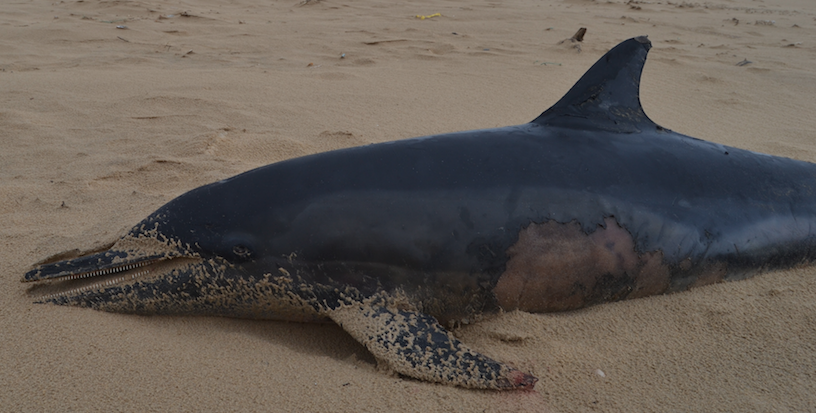
\includegraphics[width=5.5cm]{tt}
			\end{center}
		\end{figure}
	\centering \tiny \copyright Pierre-Louis Stenger
\end{frame}

\begin{frame}

	
Besoin de connaître la structure des populations

	\begin{figure}
		\begin{center}
		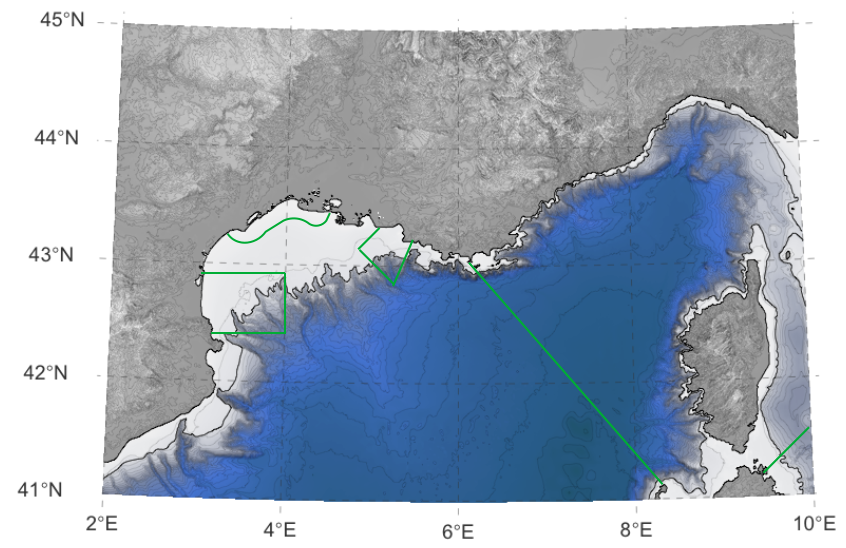
\includegraphics[width=11cm]{CarteAMPvertes}
		\end{center}
	\end{figure}
\end{frame}

\begin{frame}
	\frametitle{Points clés}
	\begin{itemize}
		\item Trou d'échantillonnage en Méditerranée
	\end{itemize}
	
	\begin{figure}
		\begin{center}
		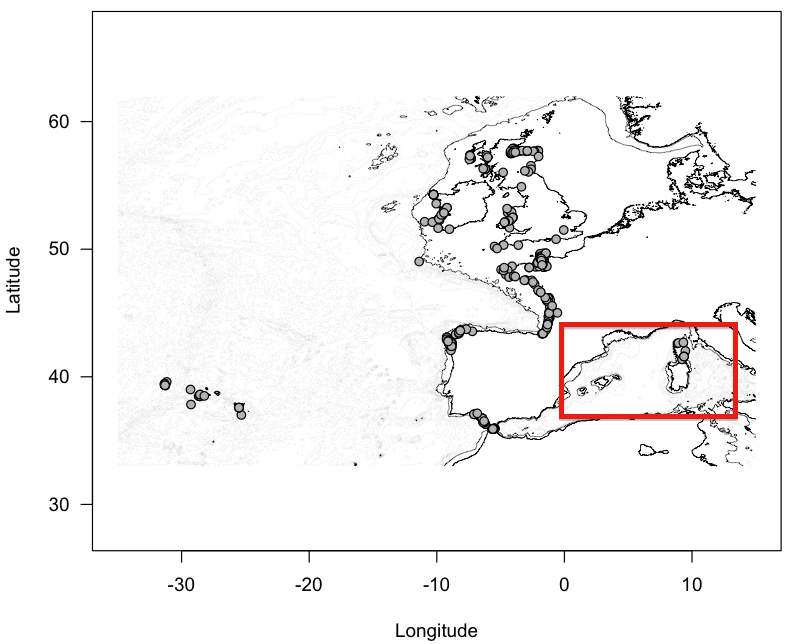
\includegraphics[width=9cm]{ML2}
		\end{center}
	\end{figure}
\end{frame}

\begin{frame}
	\frametitle{Points clés}
	\begin{itemize}
		\item  <1->Trou d'échantillonnage en Méditerranée
		\item  <1->Une seule en Méditerranée Nord Occiendale, éloignée des autres
		\item  <2->Semble être pélagique en terme de diversité génétique
		\\[5.1cm]
	\end{itemize}
\end{frame}

\section{Méthodes}


\begin{frame}
	\frametitle{Choix des marqueurs}

\begin{table}	
\begin{tabular}{lll}
  \hline
Marqueurs & Microsatellites & Mitochondriaux \\
  \hline
Nombre & 25 & 1 \\
Hérédité & Bi-parentale & Maternelle \\
Évolution & Rapide & Lente \\
  \hline
\end{tabular}
\end{table}
	
\end{frame}


%\subsection{Structure des populations}
\begin{frame}
	\frametitle{Qualité des données}
	
\begin{enumerate}
	\item ADN microsatellite
	
	\begin{itemize}
		\item $40$ individus retenus sur les $67$
	\end{itemize}
	
\end{enumerate}	
	
	\begin{figure}
		\begin{center}
		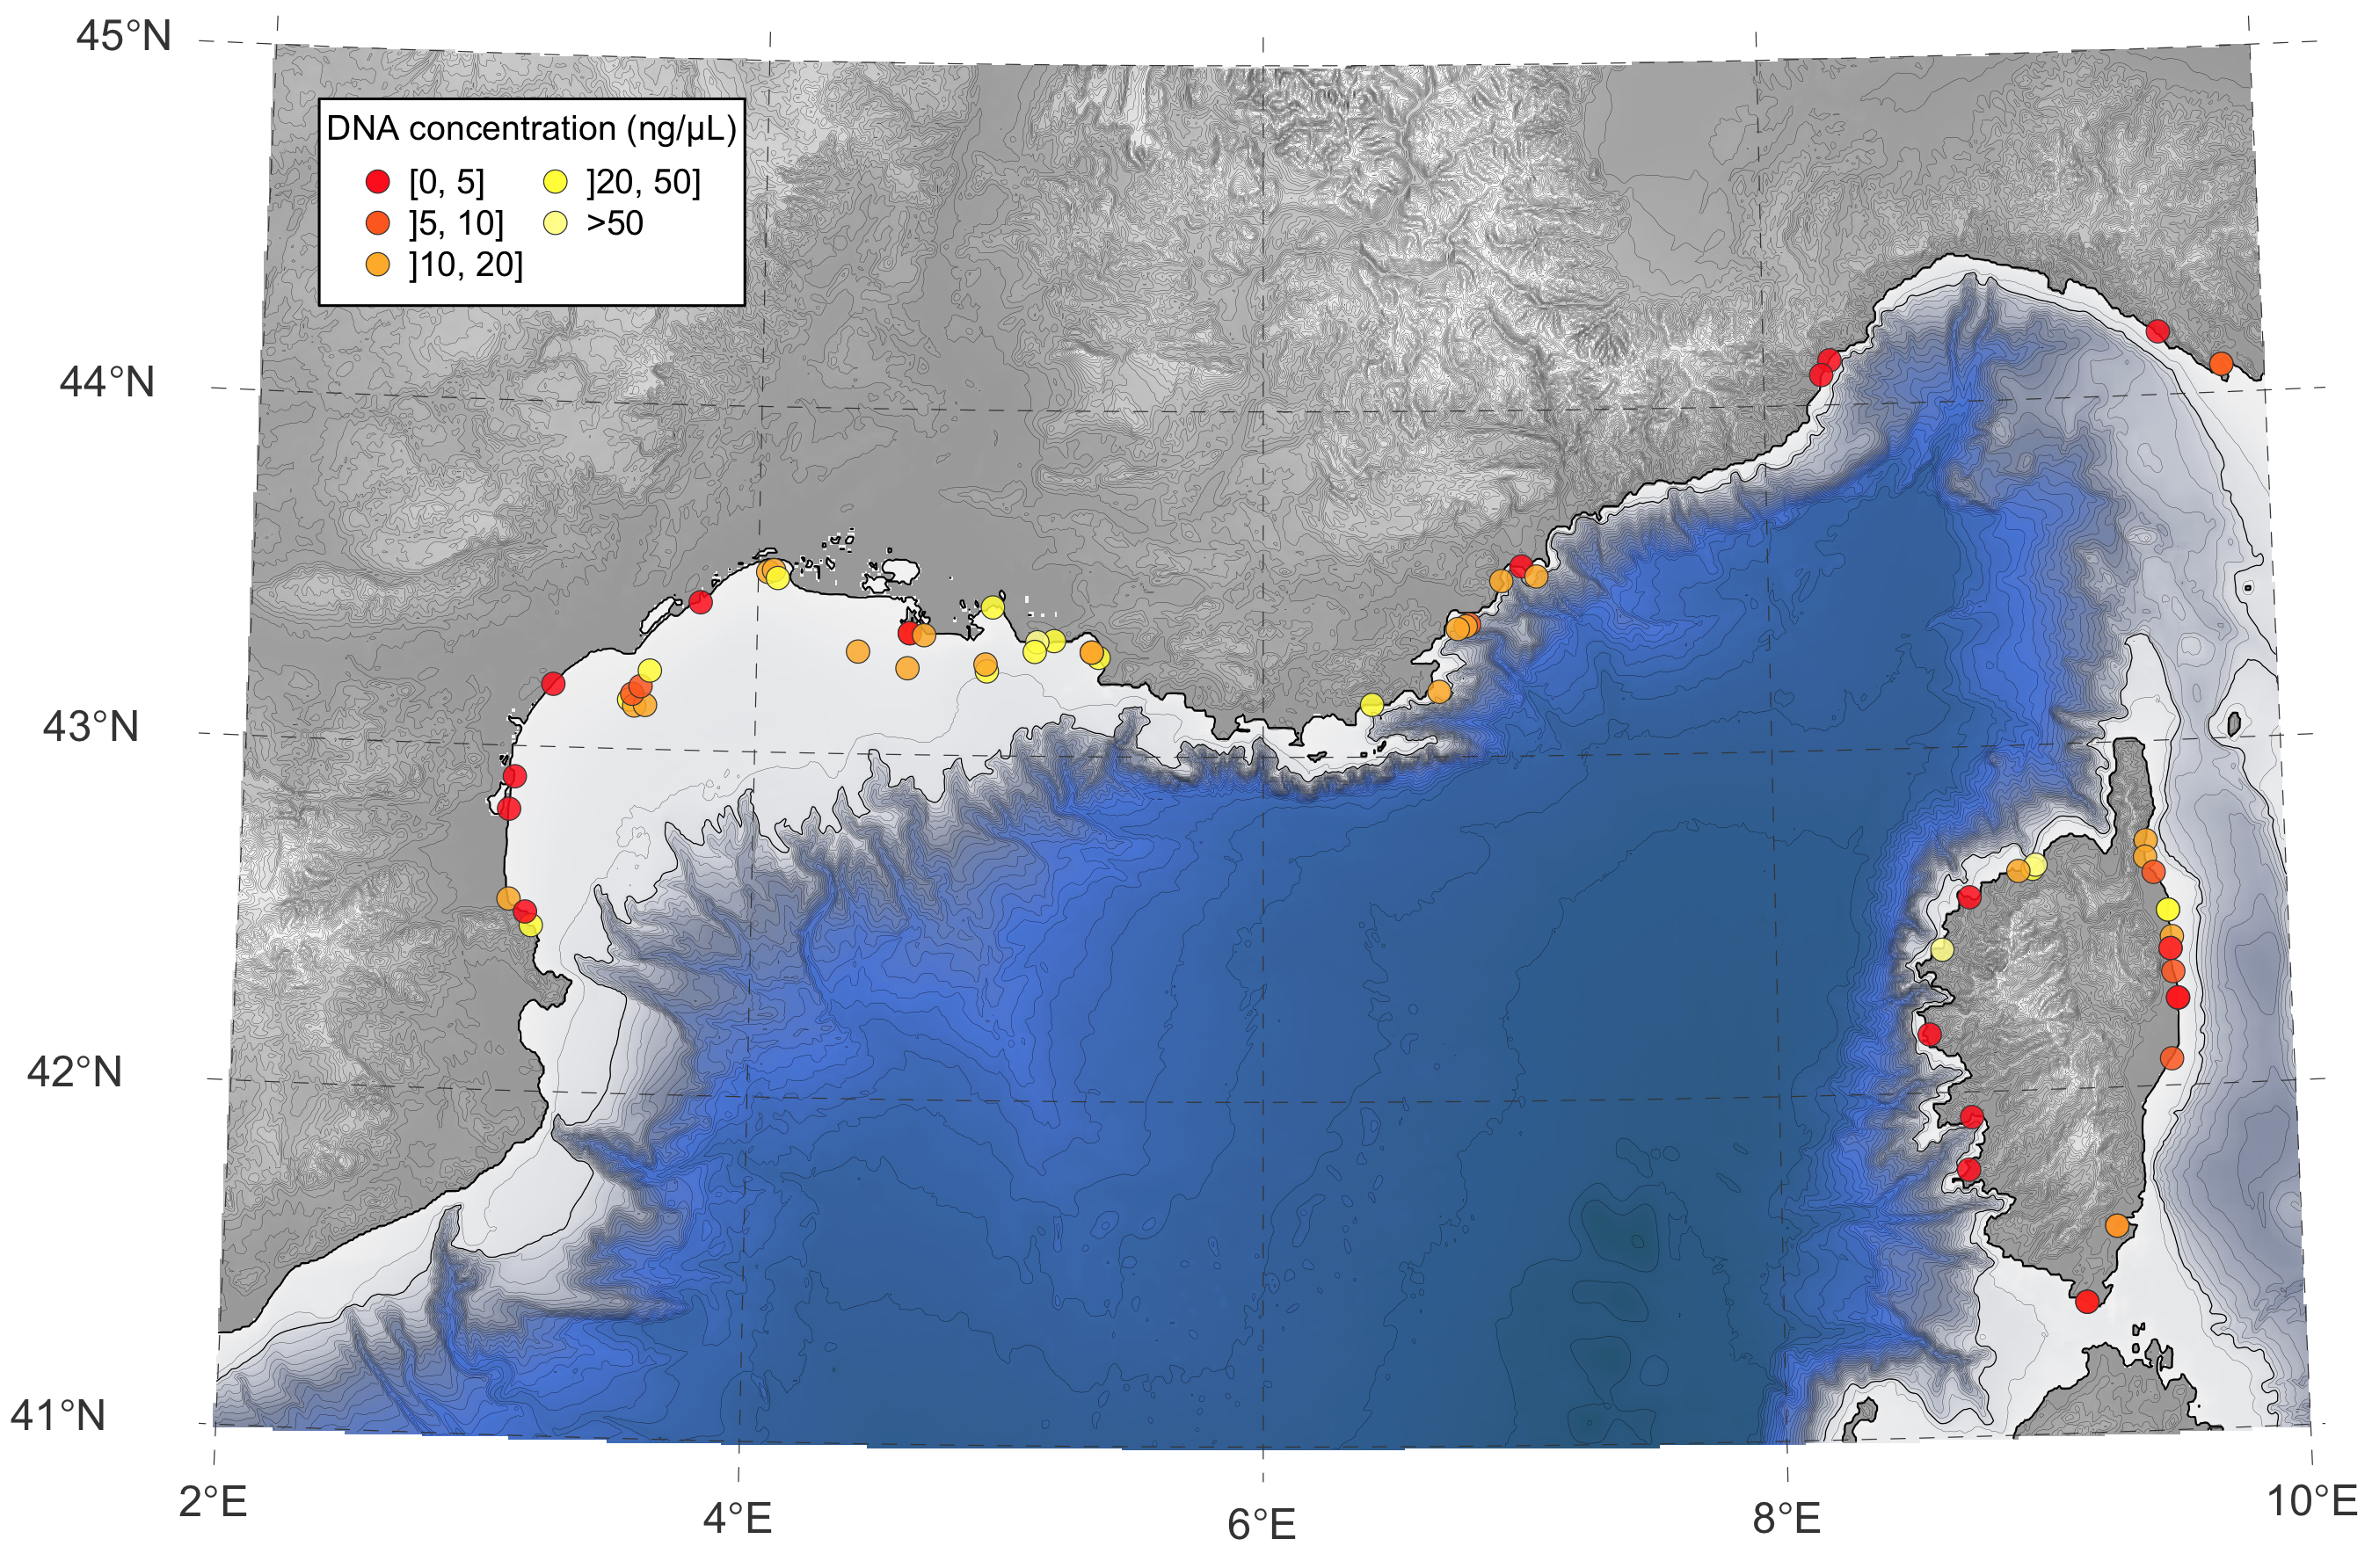
\includegraphics[width=9cm]{concentrations}
		\end{center}
	\end{figure}
\end{frame}


\begin{frame}
	\frametitle{Qualité des données}
\begin{enumerate}
	\item ADN microsatellite
	\begin{itemize}
		\item $40$ individus retenus sur les $67$
		\item $12$ marqueurs retenus sur les $25$
	\end{itemize}
\end{enumerate}
\\[6.2cm]
\end{frame}


\begin{frame}
	\frametitle{Qualité des données}
\begin{enumerate}
	\item ADN microsatellite
	\begin{itemize}
		\item $40$ individus retenus sur les $67$
		\item $12$ marqueurs retenus sur les $25$
	\end{itemize}
	\item ADN mitochondrial
	\begin{itemize}
		\item $63$ séquences de 682 pb retenues sur les $67$
	\end{itemize}
\end{enumerate}
\\[5.1cm]
\end{frame}


\begin{frame}
	\frametitle{Qualité des données}
\begin{enumerate}
	\item ADN microsatellite
	\begin{itemize}
		\item $40$ individus retenus sur les $67$
		\item $12$ marqueurs retenus sur les $25$
	\end{itemize}
	\item ADN mitochondrial
	\begin{itemize}
		\item $63$ séquences de 682 pb retenues sur les $67$
	\end{itemize}
\end{enumerate}
\\[2cm]


\begin{table}	
\begin{tabular}{cccccccc}
  \hline
  Type d'ADN & Set $1$ & Ind. de Marie Louis & Dont & Set $2$ \\
  \hline
 ADN microsatellite & 40 & 81 & 5 & 121\\
 ADN mitochondrial  & 63 & 75 & 4 & 138 \\
  \hline
\end{tabular}
\end{table}

\\[5.1cm]
\end{frame}



\section{Structure}

\begin{frame}
	\frametitle{Inférence des populations}
	\begin{figure}
		\begin{center}
		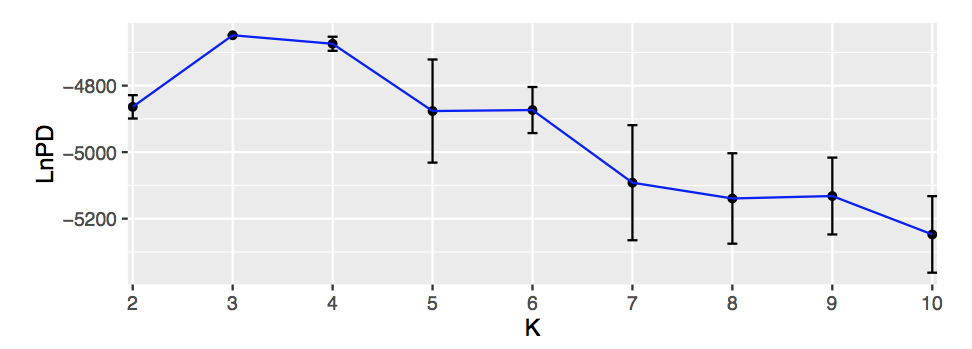
\includegraphics[width=10.5cm]{lnpd1}\\
		\small\texttt{Structure~v2.3.4} \small\citep{pritchard2000}\\[0.5cm]
		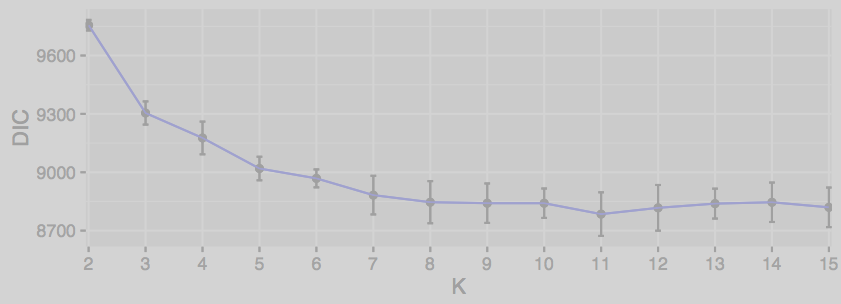
\includegraphics[width=5cm]{dic}\hspace*{0.7cm}~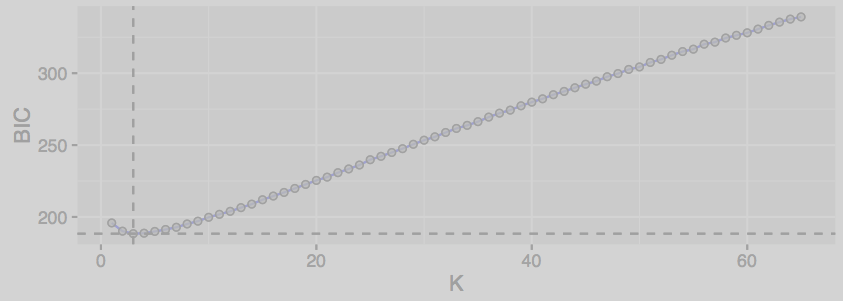
\includegraphics[width=5cm]{bic}\\
		\small\texttt{TESS~v2.3} \small\citep{durand2009}\hspace*{1.2cm}~ DAPC, \small\texttt{adegenet} \small\citep{jombart2008}
		\end{center}
	\end{figure}
\end{frame}

\begin{frame}
	\frametitle{Cartes de probabilité}
	\begin{figure}
		\begin{center}
		\hspace*{8cm}~
\includegraphics[width=0.5cm]{scale}
		\end{center}
	\end{figure}
\end{frame}


\begin{frame}
	\frametitle{Cartes de probabilité}
	\begin{columns}
	\begin{column}{0.5\textwidth}
	\begin{figure}
		\begin{center}
		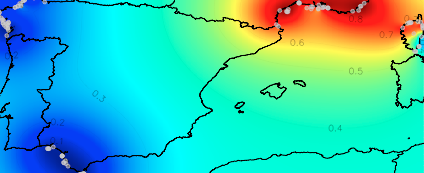
\includegraphics[width=8cm]{mno}
		\end{center}
	\end{figure}
	\end{column}
	\begin{column}{0.5\textwidth}
		\begin{figure}
			\begin{center}
			\hspace*{2cm}~
\includegraphics[width=0.5cm]{scale}
			\end{center}
		\end{figure}
		\end{column}
	\end{columns}
\end{frame}

\begin{frame}
	\frametitle{Cartes de probabilité}
	\begin{columns}
	\begin{column}{0.5\textwidth}
	\begin{figure}
		\begin{center}
		\hspace*{2cm}~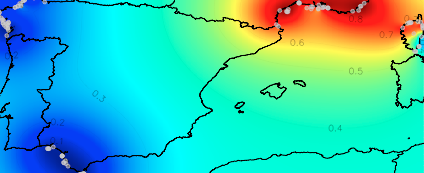
\includegraphics[width=5cm]{mno}\\[0.5cm]
		\hspace*{2cm}~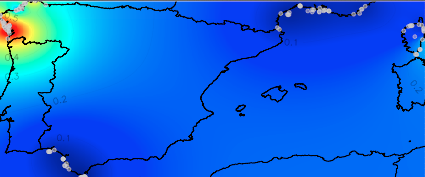
\includegraphics[width=5cm]{galice}\\[0.5cm]
		\hspace*{2cm}~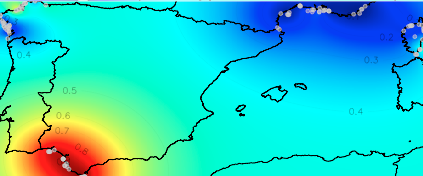
\includegraphics[width=5cm]{gib}
		\end{center}
	\end{figure}
	\end{column}
	\begin{column}{0.5\textwidth}
		\begin{figure}
			\begin{center}
			\hspace*{2cm}~
\includegraphics[width=0.5cm]{scale}
			\end{center}
		\end{figure}
		\end{column}
	\end{columns}
\end{frame}

\begin{frame}
	\frametitle{Barplot}
	\begin{figure}
		\begin{center}
		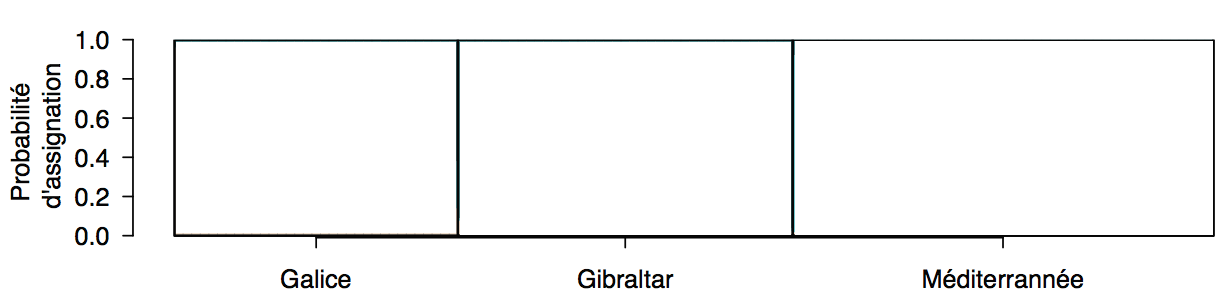
\includegraphics[width=10cm]{barplotnul}\\[0.5cm]
		
\includegraphics[width=6cm]{demileg}
		\end{center}
	\end{figure}
\end{frame}

\begin{frame}
	\frametitle{Barplot}
	\begin{figure}
		\begin{center}
		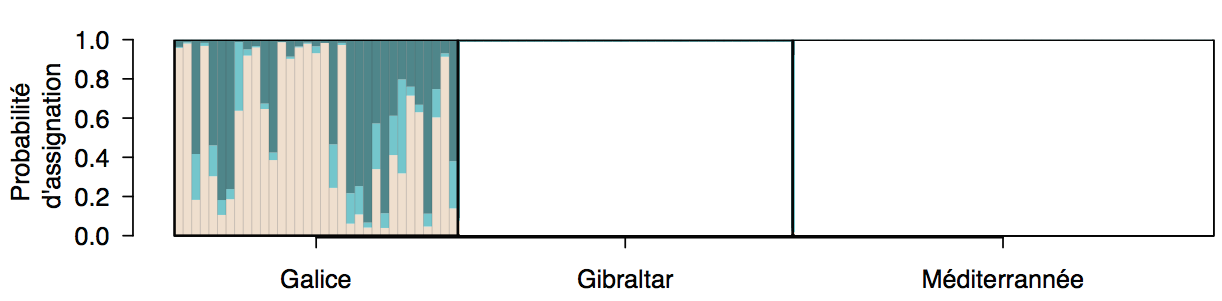
\includegraphics[width=10cm]{barplotgib}\\[0.5cm]
		
\includegraphics[width=6cm]{demileg}
		\end{center}
	\end{figure}
\end{frame}

\begin{frame}
	\frametitle{Barplot}
	\begin{figure}
		\begin{center}
		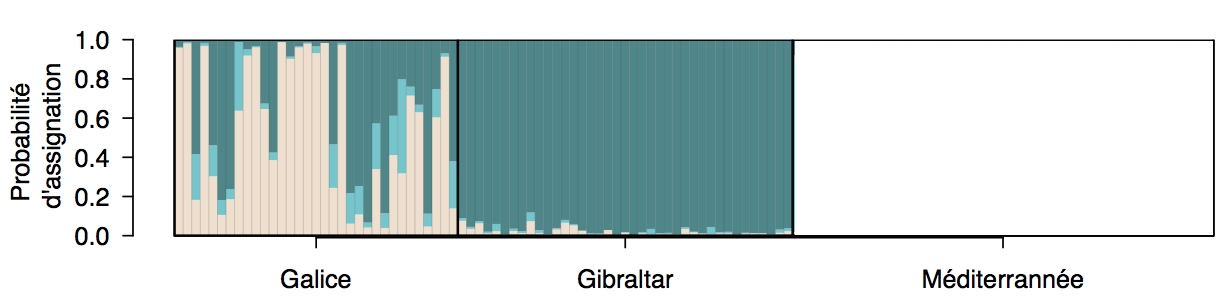
\includegraphics[width=10cm]{barplotmno}\\[0.5cm]
		
\includegraphics[width=6cm]{demileg}
		\end{center}
	\end{figure}
\end{frame}

\begin{frame}
	\frametitle{Barplot}
	\begin{figure}
		\begin{center}
		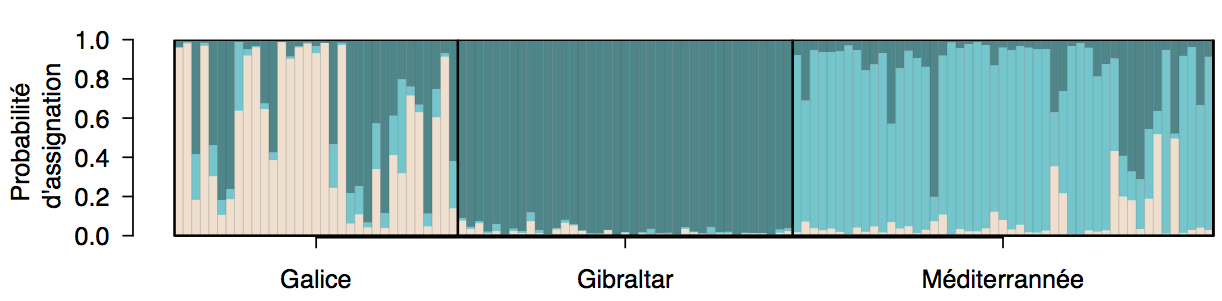
\includegraphics[width=10cm]{barplot}\\[0.5cm]
		
\includegraphics[width=6cm]{demileg}
		\end{center}
	\end{figure}
\end{frame}

\begin{frame}
	\frametitle{Barplot}
	\begin{figure}
		\begin{center}
			\\[0.5cm]
		\includegraphics[width=10cm]{barplotgris}\\[0.5cm]
		
\includegraphics[width=6cm]{demileg}
		\end{center}
	\end{figure}
\end{frame}

\begin{frame}
	\frametitle{Barplot}
	\begin{figure}
		\begin{center}
		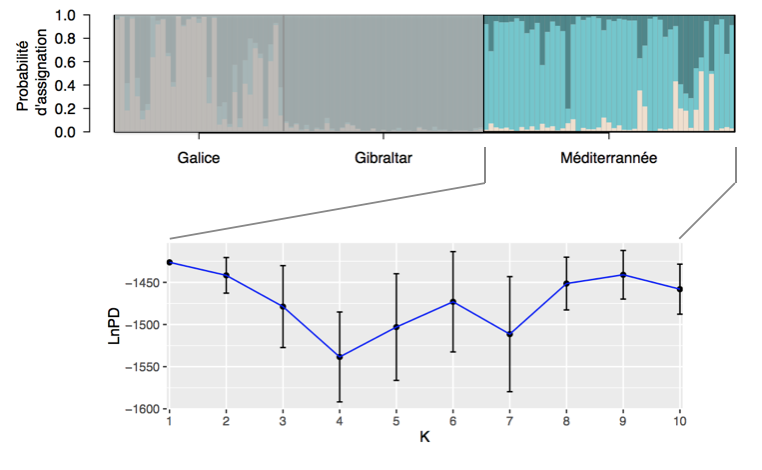
\includegraphics[width=10cm]{barln}\\[0.5cm]
		%
\includegraphics[width=6cm]{demileg}
		\end{center}
	\end{figure}
	\centering \textbg{K = 1} 	\\[2cm]
\end{frame}

\section{Caractérisation}

\begin{frame}
	\frametitle{$F_\textrm{ST}$ par paire de population}
\begin{table}[htpb]
\begin{center}
\centering
\begin{tabular}{lll}
  \hline
   &   Galice   &    Gibraltar    \\
  \hline
Gibraltar   &   0.104 * 	& - \\
MNO   &   0.139 & 0.055 ** \\
  \hline
\end{tabular}
\end{center}
\end{table}
\centering p value 0.05 = *; p value 0.01 = **; 
\end{frame}

\begin{frame}
	\frametitle{Indices synthétiques microsatellites}
	
\begin{table}[htpb]
\centering
\begin{tabular}{lllll}
\hline
 & $N$ & $F_\textrm{IS}$ & P value $F_\textrm{IS}$  & $R_{All}$ \\
\hline
Galice 			&	21	&	0.143	& 	 &	6 	\\
Gibraltar 		&	58	&	0.029	& *  &	8	\\
MNO 			&	42	&	-0.0120	& ** &	8	 \\
\hline
Global 			&	121	&	0.161	&    &	11 	\\
\hline
\end{tabular}
\end{table}
\centering $N$ : nombre d'individus, $F_\textrm{IS}$ : coefficient de consanguinité, $R_{All}$ : Richesse allélique.
\end{frame}

\begin{frame}
	\frametitle{Indices synthétiques mitochondriaux}
\begin{table}[!]
\centering
\begin{tabular}{llll}
\hline
 & $N$	&	$h$	&	$Pi$	\\
\hline
Galice &	18	&	0.562	&	0.0064 \\
Gibraltar &	52	&	0.918	&	0.0129 	\\
MNO &	39	&	0.808	&	0.0110	 \\
\hline
Global &	138	&	0.906	&	0.0128	\\
\hline
\end{tabular}
\end{table}	
\centering $N$: Nombre d'individus; $h$: Diversité haplotypique $Pi$: Diversité nucléotidique
\end{frame}

\begin{frame}
	\frametitle{Indices synthétiques mitochondriaux}
\begin{table}[!]
\centering
\begin{tabular}{rcc}
\hline
 & $N$	& $D Taj$\\
\hline
Galice &	18	 & -0.1916	\\
Gibraltar &	52	& 0.9547	\\
MNO &	39		& 0.3372 \\
\hline
Global &	138	&	0.7109	\\
\hline
\end{tabular}
\end{table}	
\centering $N$: Nombre d'individus; $D Taj$: D de Tajima
\end{frame}

\begin{frame}
	\frametitle{Réseau d'haplotypes}
	\begin{figure}
		\begin{center}
		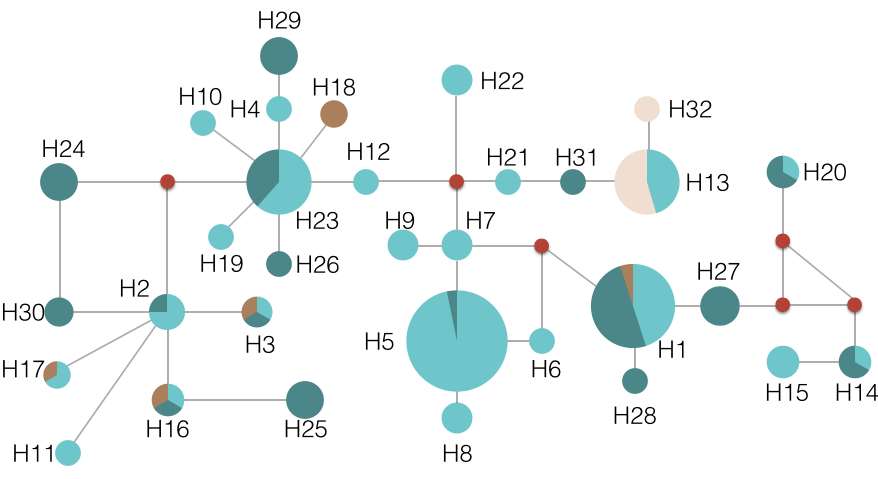
\includegraphics[width=10cm]{reseau}\\[0.5cm]
		
\includegraphics[width=8cm]{totalleg}
		\end{center}
	\end{figure}
\end{frame}

%\subsection{Sexage}
\begin{frame}
	\frametitle{Sexage}
Info sexage à mettre
\end{frame}

\section{Conclusion}

\begin{frame}
\frametitle{Discussion}
En MNO, là où il y avait un trou d'échantillonnage:
\begin{itemize}
	\item <1-> Une seule population (K=1)
	\item <2-> Relativement éloignée des autres
	\item <3-> D Tajima: Population en déclin ?
	\item <4-> Qui semble être pélagique en terme de diversité génétique \citep{lowther2014}
\end{itemize}
\end{frame}

\section{Perspectives}

\begin{frame}
\frametitle{Perspectives}
\begin{itemize}
	\item <1-> Cétacés échoués $\Rightarrow$  pas de modèle de courantologie en Mer Méditerranée \cite{peltier2012significance}
	\item <2-> Conservation
	\item <3-> Scan génomique pour adaptation locale
\end{itemize}
\end{frame}

\begin{frame}
\frametitle{Merci pour votre attention}
		\begin{figure}
			\begin{center}
			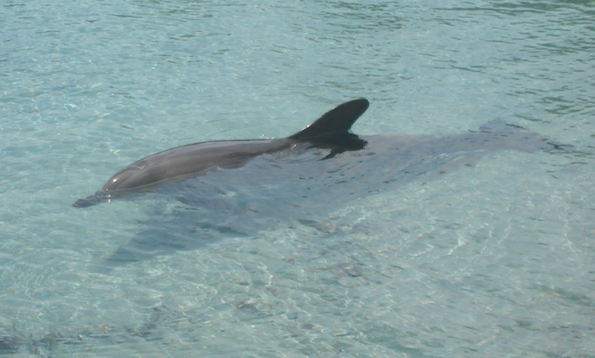
\includegraphics[width=7cm]{tursiopsAussie} 
			\end{center}
		\end{figure}
		\centering \tiny\copyright Pierre-Louis Stenger
\end{frame}

\begin{frame}[allowframebreaks]
	\bibliographystyle{newbst}
	\footnotesize\bibliography{Bibliographie}
\end{frame}

\begin{frame}
	\frametitle{Trois méthodes}
	\begin{figure}
		\begin{center}
		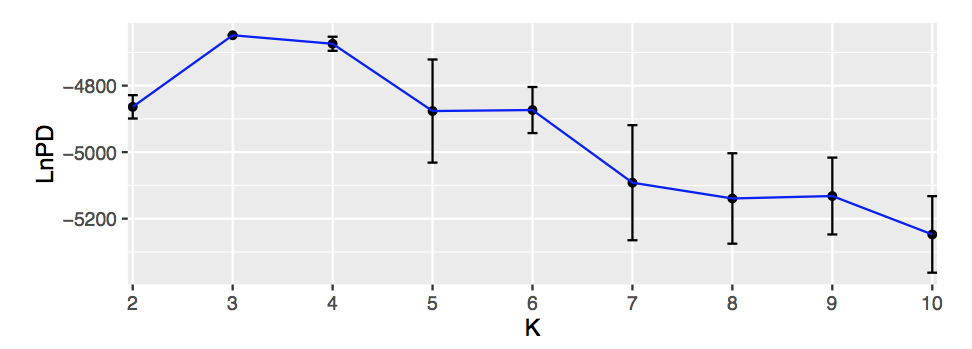
\includegraphics[width=11.5cm]{lnpd1}
	
		\end{center}
	\end{figure}
\end{frame}

\begin{frame}
	\frametitle{Trois méthodes}
	\begin{figure}
		\begin{center}
		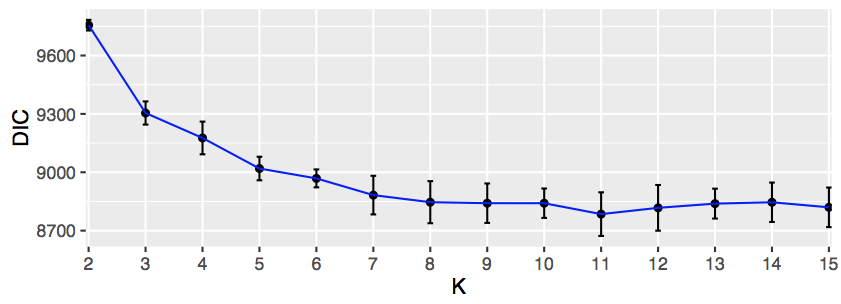
\includegraphics[width=11cm]{dic2}
		
		\end{center}
	\end{figure}
\end{frame}

\begin{frame}
	\frametitle{Trois méthodes}
	\begin{figure}
		\begin{center}
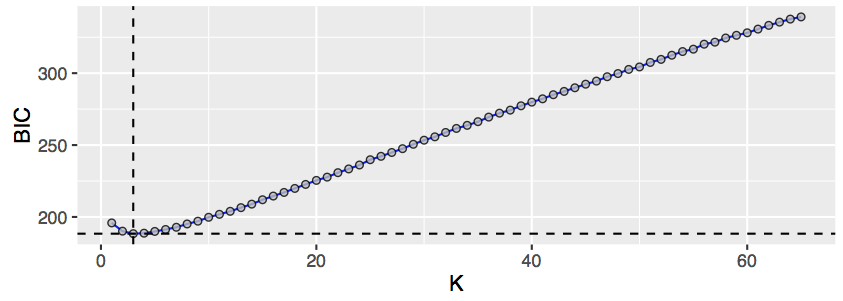
\includegraphics[width=11cm]{bic2}
		
		\end{center}
	\end{figure}
\end{frame}

\begin{frame}
\frametitle{Discussion}
\begin{itemize}
		\item Une population galicienne
			\begin{itemize}
				\item Population pélagique \citep{louis2014}
				\item Population côtière \citep{louis2014} 
			\end{itemize}
	\item Une population de Gibraltar 
	\begin{itemize}
		\item Pélagiques ? \citep{lowther2014}
	\end{itemize}
	\item Une population en MNO
	\begin{itemize}
		\item Pélagiques ? \citep{lowther2014}
	\end{itemize}
\end{itemize}
\end{frame}

\end{document}

